%---------------------------------------------------------
\section{Description}
IzPack est un projet open-source créé en 2001 par Julien Ponge.
C'est un générateur d'installateur et il présente à ce titre de nombreuses fonctionnalités.
\subsection{Générateur d'installateur}
Une application, une fois réalisée, nécessite un certain nombre d'opérations sur la machine pour être opérationnelle.
Ces opérations vont de la décompression de l'archive dans un répertoire au lancement de scripts de configuration en passant par la validation de la licence et la création de raccourcis.
Créer un installateur pour une application est souvent laborieux et chronophage mais nécessaire, étant donné qu'il apparaît comme le premier contact avec l'utilisateur et joue beaucoup sur son jugement.

L'intérêt d'IzPack réside dans le fait qu'il propose une solution pour créer cet installateur de manière simple et universelle.
En effet, à partir d'une application existante, IzPack est capable de générer un installateur pour cette application.
Ce dernier pourra être utilisé pour déployer l'application sur n'importe quelle machine.
De plus, tout type de programme peut être packagé, que ce soit une application C++ ou Java. IzPack se chargeant juste de la logique d'installation, il est totalement independant du contenu qu'il installe.
\subsection{Open-source}
Le projet IzPack est un projet open-source sous la fondation Codehaus.
A ce titre, le code source est librement accessible selon les termes de la licence. De plus, une communauté s'est regroupée autour du projet.
\subsubsection{Codehaus}
Codehaus est une fondation dédiée au développement de projets open-source.
A ce titre, elle propose une plateforme pour aider au développement de ces projets avec un certain nombre d'outils fournis par des sponsors.
Par exemple, Atlassian fournit pour les projets leur système de suivie de bug, JIRA, JetBrain fournit une licence IntelliJ, etc...
\subsubsection{Structure de la communauté}
Les projets sous Codehaus sont des méritocraties.
Un despote supervise un projet et
les développeurs désirant rejoindre un projet doivent apporter une contribution, montrer leur motivation et être approuvés par le despote.
En général, les décisions se prennent de manière démocratique pour tout ce qui concerne le projet.

Une mailing-list pour les développeurs permet de communiquer les informations et prendre les décisions d'un commun accord.
Pour éviter tout blocage dans les décisions, le despote a toujours le dernier mot.

Dans le cas de IzPack, le despote est Julien Ponge.
\subsubsection{La communauté IzPack}
Cette communauté open-source fait vivre et évoluer le projet. Les personnes rejoignant le projet sont des personnes aux motivations diverses.
Ces personnes peuvent être des passionnés intéressés par le projet ou des salariés utilisant IzPack et apportant leurs contributions.
Ces formes de contributions sont variées, 
elles peuvent prendre la forme d'aide aux utilisateurs, de rédaction de documentation, de correction de bugs ou d'ajouts de fonctionnalités.
\subsubsection{Licence Apache 2}
IzPack est sous licence Apache 2. Cette licence permet l'accès au code source et l'utilisation libre du logiciel.
Il est tout à fait possible de l'utiliser pour une application commerciale, voire même de modifier les sources pour le faire correspondre à ses besoins.

Si un développeur apporte des modifications utiles, il est encouragé à en faire profiter la communauté, mais ce n'est pas une obligation.
\subsection{Fonctionnalités}
IzPack est un système modulaire, il possède de nombreuses fonctionnalités pour créer un installateur adapté à chacun.
\subsubsection{Multi-plateforme}
L'installateur généré par IzPack est un jar (java archive).
Il suffit donc que la machine ait une machine virtuelle pour pouvoir lancer l'installation, indépendamment de la plateforme ou du système d'exploitation.
Il est néanmoins possible de faire des traitements spécifiques à certaines plateformes, par exemple créer des raccourcis sous Windows et modifier la base de registre, modifier le PATH sous Linux...
Il est également possible de convertir l'installateur pour être spécifique à une plateforme.
\subsubsection{Personnalisation}
Chaque écran que verra l'utilisateur est décrit par un panel.
Un ensemble de panels composent l'installateur graphique et chaque panels remplit une fonction spécifique.
L'aspect global de l'installateur et celui des panels est personnalisable par l'utilisateur via le descripteur XML.
\begin{figure}[H]
	\centering
	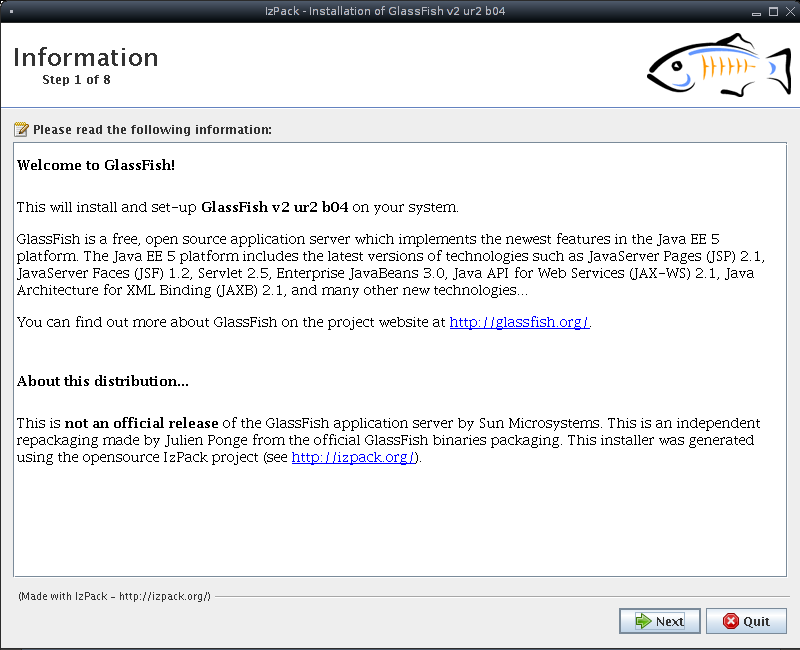
\includegraphics[width=0.3\textwidth]{../dia/included/install/02.png}
	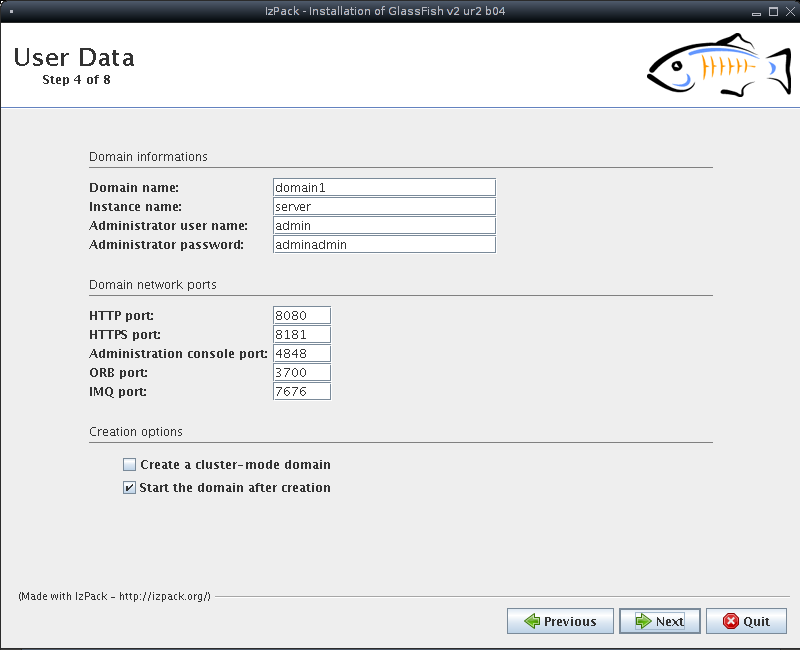
\includegraphics[width=0.3\textwidth]{../dia/included/install/05.png}
	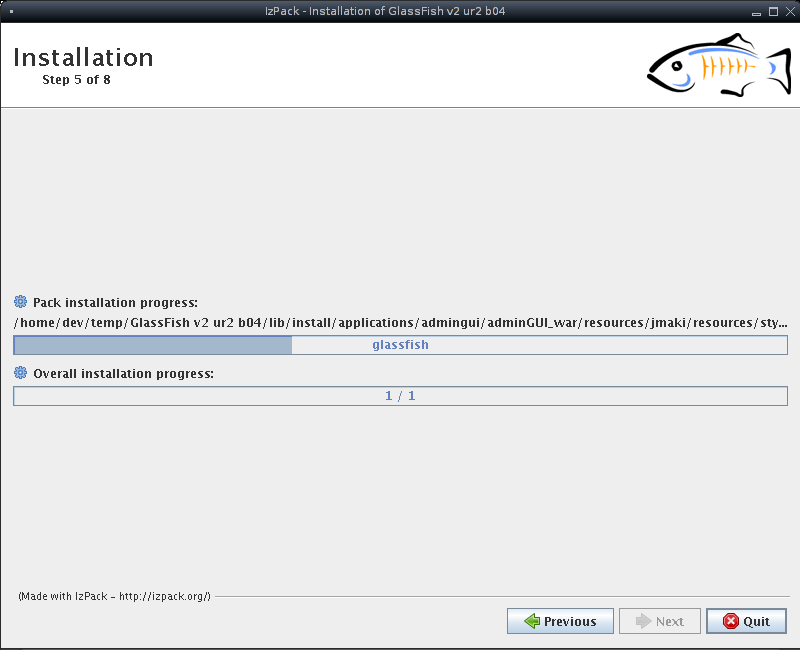
\includegraphics[width=0.3\textwidth]{../dia/included/install/06.png}
	\caption{Exemple de panels disponibles avec IzPack}
	\label{fig:panelGlass}
\end{figure}
Il existe de nombreux types de panels : des panel pour accueillir l'utilisateur et lui afficher des informations (HelloPanel et HTMLInfoPanel), d'autres pour demander à l'utilisateur des informations (UserInputPanel), etc...

Sur la figure~\ref{fig:panelGlass}, on peut voir un HTMLInfoPanel, un UserInputPanel et un InstallPanel pour l'installation de Glassfish.
Il existe aussi des panels plus spécialisés comme CompilePanel qui permet de compiler du code java et ProcessPanel qui permet de lancer des programmes après l'installation.
\subsubsection{Internationalisation}
IzPack supporte la création d'installateurs multilangues (voir figure \ref{fig:LangChoice}).
Pour la localisation, tout repose sur des fichiers XML.
Si une langue n'existe pas, il suffit de traduire le dictionnaire correspondant dans un fichier XML et de l'utiliser lors de la création de l'installateur.
\begin{figure}[H]
	\centering
	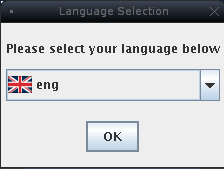
\includegraphics[width=5cm]{../image/LangChoice.png}
	\caption{Exemple de choix de langue avec IzPack}
	\label{fig:LangChoice}
\end{figure}
\subsubsection{Installation automatique}
A la fin de l'installation, il est possible de générer un script d'installation automatique comme montré figure \ref{fig:SaveInstallXML}.
Ce script permet de reproduire l'installation qui vient d'être réalisée sur d'autres machines.
\begin{figure}[H]
	\centering
	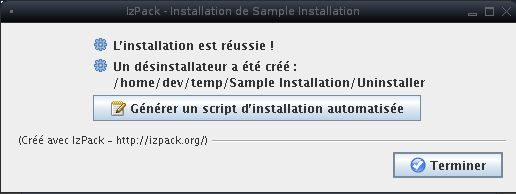
\includegraphics[width=12cm]{../image/SaveInstallXML.png}
	\caption{Fin d'installation, enregistrement du script d'installation automatisé}
	\label{fig:SaveInstallXML}
\end{figure}
\subsection{Popularité du projet}
IzPack est utilisé dans de grand projets comme Jboss, Xwiki, Glassfish... Des entreprises également l'utilisent pour leurs propres applications. A l'heure actuelle, les téléchargements mensuels s'élèvent à 25.000.
\begin{figure}[H]
	\centering
	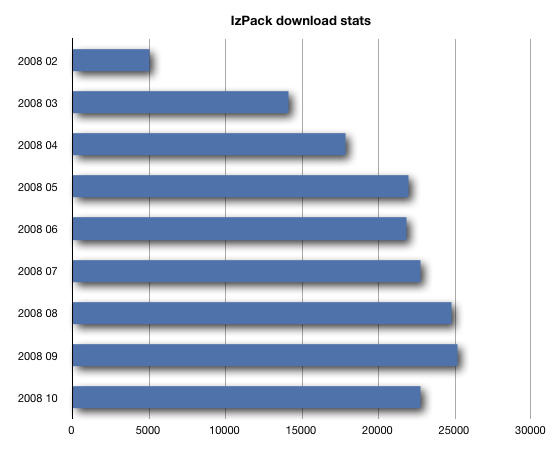
\includegraphics[width=0.6\textwidth]{../image/telechargements.png}
	\caption{Statistiques de téléchargements}
\end{figure}
 %---------------------------------------------------------
\section{Architecture}
Globalement, IzPack possède 2 composants, le compilateur qui va gérer la création de l'installateur et l'installateur lui-même.

\subsection{Compilateur}
Le compilateur se charge de packager l'ensemble des fichiers nécessaires dans un seul fichier jar.
Ces fichiers comprennent l'application en elle-même et les fichiers nécessaires (les panels décrits dans le XML, etc) à l'installation.
Cette partie est utilisée par le développeur qui souhaite créer un installateur.

\subsection{Installateur}
La partie installation concerne toute la logique et la présentation du processus d'installation. Cette partie sera exécutée par un utilisateur souhaitant installer le logiciel.
\subsection{Utilisation}
Dans un premier temps, le compilateur va créer l'installateur de l'application.
Il prend la partie installation d'IzPack, la modifie pour correspondre à l'installation décrite dans le fichier XML, et la package avec l'application à installer. Cette phase est illustrée par la figure \ref{fig:partie_compil}
A noter qu'aucun IzPack n'a été blessé lors de la compilation.
%TODO On laisse ca????
\begin{figure}[H]
	\centering
	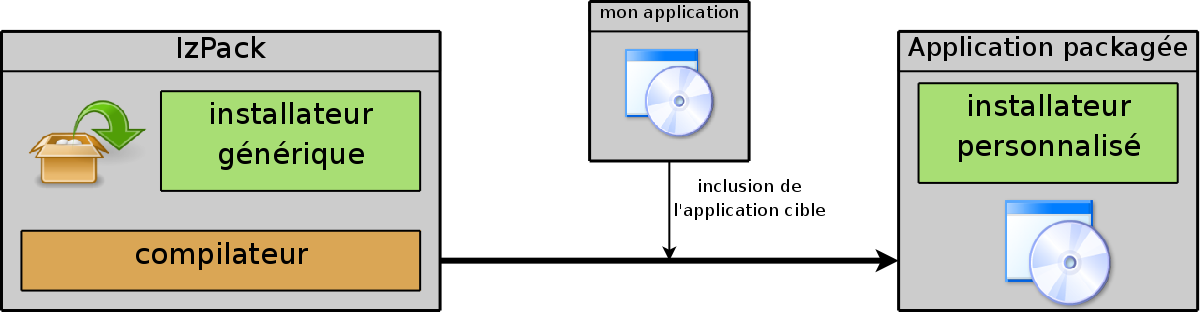
\includegraphics[width=\textwidth]{../image/partie_compil.png}
	\caption{Phase de compilation}
	\label{fig:partie_compil}
\end{figure}

Cette application est alors prête à être déployée sur une autre machine.
Le processus d'installation est géré par la partie installateur de IzPack.
Cette phase, illustrée par la figure \ref{fig:partie_install}, va permettre de déployer l'application sur toutes les machines nécessaires.
\begin{figure}[H]
	\centering
	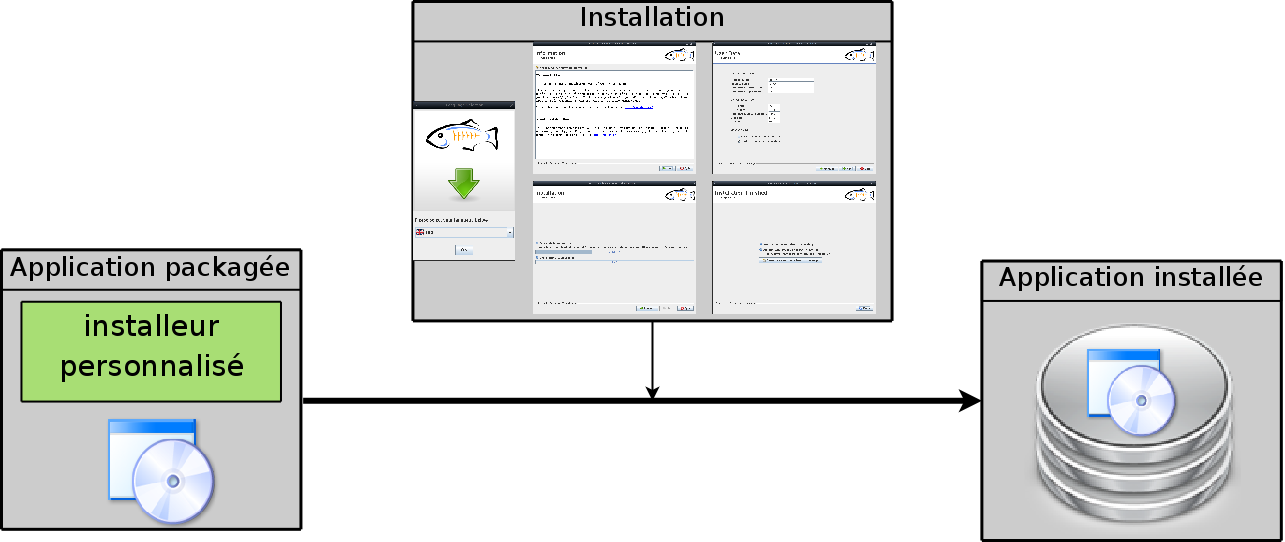
\includegraphics[width=\textwidth]{../image/partie_install.png}
	\caption{Phase d'installation}
	\label{fig:partie_install}
\end{figure}

%---------------------------------------------------------
\section{Exemple d'installation}
Des exemples complets de génération d'installation existent.
Il suffit de récupérer les sources d'un projet open-source utilisant IzPack comme IzPack, Glassfish, PerfSonar, Xwiki... 
Pour illustrer simplement l'utilisation de IzPack, utilisons plutôt le petit exemple fourni avec le code de l'application.
\subsection{Description du XML}
Ce XML (install.xml) décrit complètement l'installation.
Une balise \verb|info| permet de définir les informations concernant l'application :
\begin{lstlisting}[language=XML]
<info>
	<appname>Sample Installation</appname>
	<appversion>1.4 beta 666</appversion>
	...
</info>
\end{lstlisting}
Une autre balise, \verb|guipref| permet de définir quelques propriétés de la fenêtre de l'installateur :
\begin{lstlisting}[language=XML]
<guiprefs width="640" height="480" resizable="yes"/>
\end{lstlisting}
Les langues sont définies par la balise \verb|locale| :
\begin{lstlisting}
<locale>
	<langpack iso3="eng"/>
	<langpack iso3="fra"/>
</locale>
\end{lstlisting}
Des fichiers externes nécessaires à l'installation peuvent être définis par la balise \verb|resources| :
\begin{lstlisting}[language=XML]
<resources>
	<res id="LicencePanel.licence" src="Licence.txt"/>
</resources>
\end{lstlisting}
Les panels visibles par l'utilisateur sont décrits dans la balise \verb|panels| :
\begin{lstlisting}[language=XML]
<panels>
	<panel classname="HelloPanel"/>
	...
	<panel classname="FinishPanel"/>
</panels>
\end{lstlisting}
Enfin la balise \verb|packs| contient la description des paquets (les différentes parties, optionnelles ou non, de l'application) à installer.
\begin{lstlisting}[language=XML]
<packs>
	<pack name="Base" required="yes">
		<description>The base files</description>
		<file src="Readme.txt" targetdir="$INSTALL_PATH"/>
		...
	</pack>
	<pack name="Docs" required="no">
		...
	</pack>
	...
</packs>
\end{lstlisting}
Bien sûr d'autres options existent, mais celles présentées ici suffisent à créer notre installateur.
Les fichiers référencés doivent être présents dans le chemin indiqué par le XML lors de la compilation.
\subsection{Génération du jar}
Pour générer notre installateur, il suffit de lancer la commande suivante : (l'exécutable \verb|compile| provient de IzPack)
\begin{verbatim}
$ compile install.XML
.::  IzPack - Version 4.1.0 ::.

< compiler spécifications version: 1.0 >

- Copyright (c) 2001-2008 Julien Ponge
- Visit http://izpack.org/ for the latest releases
- Released under the terms of the Apache Software License version 2.0.

-> Processing  : install.XML
-> Output      : install.jar
-> Base path   : .
-> Kind        : standard
-> Compression : default
-> Compr. level: -1
-> IzPack home : .

...

Build time: Tue Mar 10 16:50:27 CET 2009
\end{verbatim}
Cette exécution va produire un fichier install.jar : notre installateur.
\subsection{Installation}
Il suffit désormais de lancer le jar pour installer notre application.
\begin{figure}[H]
	\centering
	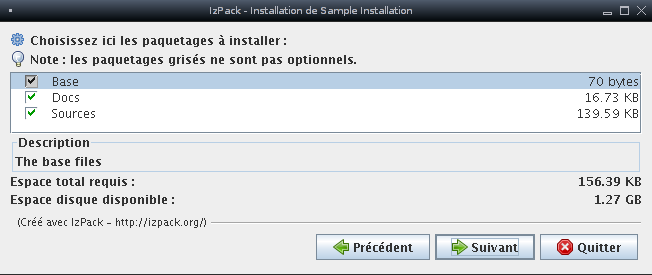
\includegraphics[width=15cm]{../image/installSample.png}
	\caption{Exemple d'installation avec IzPack}
\end{figure}
\subsection{Installation automatique}
En lançant l'installateur avec un script d'installation automatisée en paramètre, l'installation est rejouée à l'identique automatiquement.
\begin{verbatim}
$ java -jar install.jar automated.xml
[ Starting automated installation ]
[ Starting to unpack ]
[ Processing package: Base (1/3) ]
[ Processing package: Docs (2/3) ]
[ Processing package: Sources (3/3) ]
[ Unpacking finished ]
[ Writing the uninstaller data ... ]
[ Automated installation done ]
\end{verbatim}

 %---------------------------------------------------------
\section{Problèmes actuels}
IzPack possède, comme tout logiciel, des bugs potentiels ou des améliorations à effectuer.
\subsection{Code obsolète}
IzPack a débuté en 2001.
A cette époque, la Jdk en était à la version 1.2. Il y avait donc des fonctionnalités absentes comme la généricité.
On trouve ainsi, encore maintenant, du code utilisant de vieilles structures de données (des tableaux d'objets ou des Vectors) ou des styles de programmation abandonnés.
\subsection{NanoXML}
Une amélioration possible concerne la gestion des XML, qui ont une grande importance dans IzPack.
L'absence de processeur XML intégré à la JRE 1.2 a forcé l'utilisation d'une librairie externe pour traiter les documents XML.
IzPack se base donc sur une telle librairie : NanoXML.

Cette librairie n'est malheureusement plus mise à jour (la dernière mise à jour date de 2003) et possède un certains nombres de bugs.
De plus, l'environnement java (JRE) possède depuis la version 1.4 une bibliothèque native pour gérer les XML.
Se débarrasser de la dépendance à NanoXML et se reposer uniquement sur la JRE permettrait donc non seulement de rendre la gestion des XML plus sûre et robuste, mais également de diminuer la taille des installateurs générés.